\documentclass[aspectratio=169]{beamer}
\usepackage{color,amsmath}
\usepackage{subfigure}
\usepackage{booktabs}
\usepackage{framed}
\usepackage{comment}
\usepackage{ulem}

\usepackage{hyperref}
\hypersetup{
    colorlinks=true,
    linkcolor=blue,
    filecolor=magenta,      
    urlcolor=cyan,
}

%%%%%%%%%%%%%%%%%%%%%%%%%%
\title[]{[Introduction to mass collaboration]. [Human computation], [Open call], [Distributed data collection], [Fragile Families Challenge]}
\author[]{Matthew J. Salganik\\Department of Sociology\\Princeton University}
\date[]{%Summer Institutes in Computational Social Science\\2020
%\vfill
%\begin{flushleft}
%{\scriptsize
%The Summer Institutes in Computational Social Science is supported by grants from the Russell Sage Foundation and the Alfred P. Sloan Foundation.}
%\end{flushleft}
\begin{flushright}

\includegraphics[width=0.1\textwidth]{figures/cc-by.png}
\end{flushright}
}
\begin{document}
%%%%%%%%%%%%%%%%%%%%%%%%%%
\frame{\titlepage}
%%%%%%%%%%%%%%%%%%%%%%%%%%
\begin{frame}

\begin{columns}
\begin{column}{.40\textwidth}
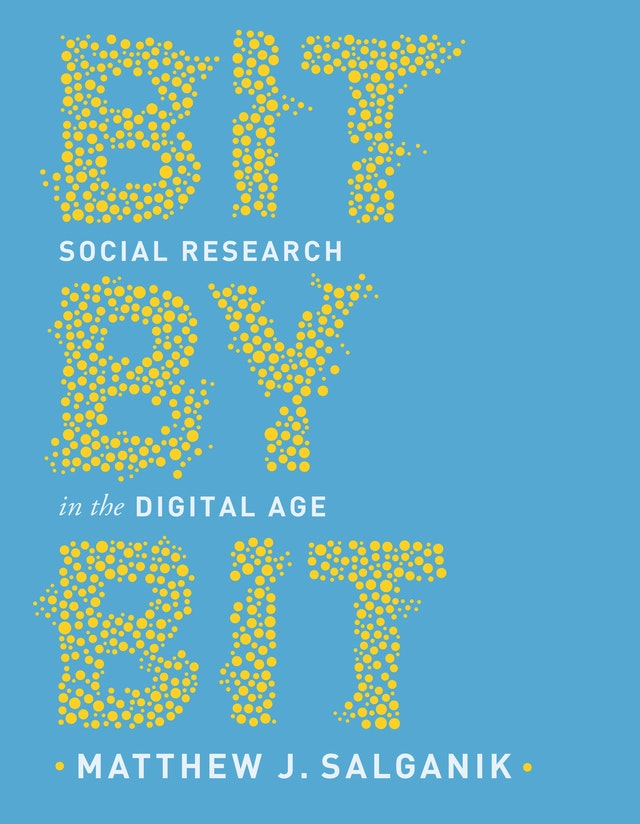
\includegraphics[width=\textwidth]{figures/salganik_bit_2018_cover}
\end{column}%

\hfill%

\begin{column}{.60\textwidth}
1) Introduction \\
2) Observing behavior \\
3) Asking questions \\
4) Running experiments \\
\textcolor{blue}{5) Mass collaboration} \\
6) Ethics \\
7) The future \\
\end{column}%
\end{columns}

\end{frame}
%%%%%%%%%%%%%%%%%%%%%%%%%
\begin{frame}

\begin{center}
\includegraphics[width=0.5\textwidth]{figures/wikipedia_logo}
\end{center}

\end{frame}
%%%%%%%%%%%%%%%%%%%%%%%%%%
\begin{frame}

Mass collaboration combines ideas from 
\begin{itemize}
\item crowdsourcing
\item citizen science
\item collective intelligence
\end{itemize}

\end{frame}
%%%%%%%%%%%%%%%%%%%%%%%%%%%
\begin{frame}

\begin{center}
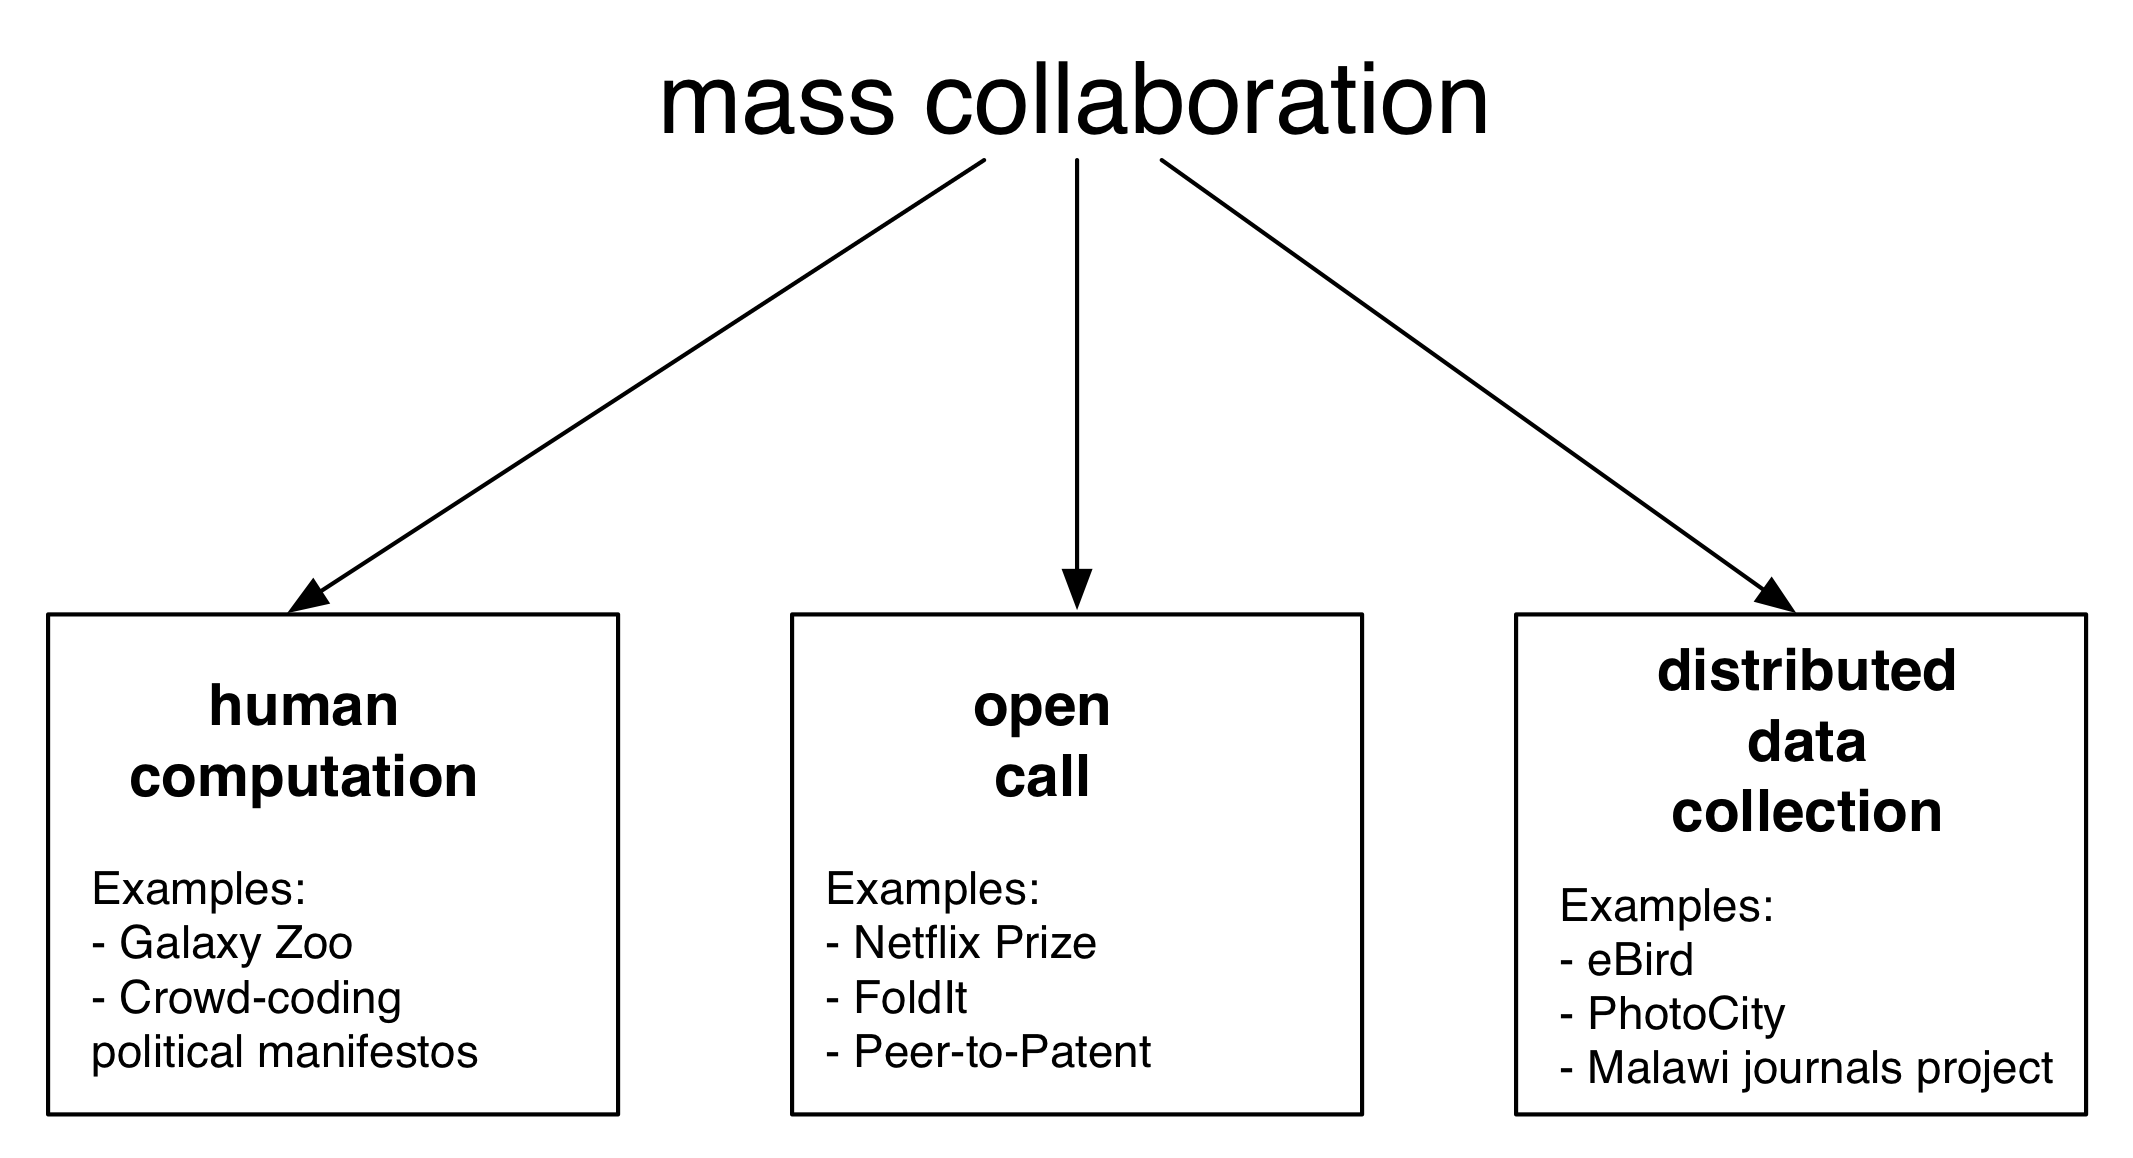
\includegraphics[width=\textwidth]{figures/mass_collaboration_schematic}
\end{center}

\end{frame}
%%%%%%%%%%%%%%%%%%%%%%%%%%
\begin{frame}

Guiding idea:\\
Collaborators not cogs (ornithology and astronomy are examples)

\end{frame}
%%%%%%%%%%%%%%%%%%%%%%%%%%
\begin{frame}

\begin{itemize}
  \item\only<1>{Is this really research?} \only<2->{\sout{Is this really research?}}
  \item<2-> Does this enable new research?
\end{itemize}

\end{frame}
%%%%%%%%%%%%%%%%%%%%%%%%%%
\begin{frame}

\begin{itemize}
  \item \only<1>{Is this perfect?} \only<2->{\sout{Is this perfect?}}
  \item<2-> Is this better than we can do without mass collaboration?
\end{itemize}

\end{frame}
%%%%%%%%%%%%%%%%%%%%%%%%%%
\begin{frame}

\begin{itemize}
  \item \only<1>{Is this impossible?} \only<2>{\sout{Is this impossible?}}
  \item<2-> Is this possible?
\end{itemize}

\end{frame}
%%%%%%%%%%%%%%%%%%%%%%%%%%
\begin{frame}

An honest assessment: \pause As far as I can tell, most mass collaborations fail

\end{frame}
%%%%%%%%%%%%%%%%%%%%%%%%%%
\begin{frame}

\begin{itemize}
\item Human computation
\item \textcolor{blue}{Open call}
\item Distributed data collection
\end{itemize}

\end{frame}
%%%%%%%%%%%%%%%%%%%%%%%%%%
\begin{frame}

\begin{center}
\includegraphics[width=0.3\textwidth]{figures/sobel_longitude_2007_cover}
\end{center}

\end{frame}
%%%%%%%%%%%%%%%%%%%%%%%%%%
\begin{frame}

{\Large
\begin{center}
Solutions are easier to check than to generate
\end{center}
}

\end{frame}
%%%%%%%%%%%%%%%%%%%%%%%%%%
\begin{frame}

{\Large
\begin{center}
You will participate in an open call in a few moments
\end{center}
}

\end{frame}
%%%%%%%%%%%%%%%%%%%%%%%%%%
\begin{frame}

{\Large
\begin{center}
Questions? 
\end{center}
}

\end{frame}
%%%%%%%%%%%%%%%%%%%%%%%%%%
\begin{frame}

\begin{itemize}
\item Human computation
\item Open call
\item \textcolor{blue}{Distributed data collection}
\end{itemize}

\end{frame}
%%%%%%%%%%%%%%%%%%%%%%%%%%
\begin{frame}

\begin{itemize}
\item people can be where the researchers can't
\pause
\item scale that researcher cannot match
\pause
\item sometimes hard to separate from human computation
\end{itemize}

\end{frame}
%%%%%%%%%%%%%%%%%%%%%%%%%%
\begin{frame}

\begin{center}
\includegraphics[width=0.6\textwidth]{figures/photocity_logo}
\end{center}

\small{
Tuite et al. (2011) ``PhotoCity: Training Experts at Large-scale Image Acquisition Through a Competitive Game'' \textit{CHI}:  \url{http://dx.doi.org/10.1145/1978942.1979146}
}

\end{frame}
%%%%%%%%%%%%%%%%%%%%
\begin{frame}

\begin{center}
\includegraphics[width=0.6\textwidth]{figures/rome_in_a_day}
\end{center}
Rome in a Day (Agarwal et al., 2009)

\end{frame}
%%%%%%%%%%%%%%%%%
\begin{frame}

\begin{center}
\includegraphics[width=0.6\textwidth]{figures/tuite_photocity_2011_fig2}
\end{center}

Two campuses: University of Washington and Cornell University

\end{frame}
%%%%%%%%%%%%%%%%%
\begin{frame}

Over 2 months, 100,000 photos submitted by 45 players
\vfill
\begin{center}
\includegraphics[width=0.9\textwidth]{figures/tuite_photocity_2011_fig8}
\end{center}

\end{frame}
%%%%%%%%%%%%%%%%%
\begin{frame}
\frametitle{PhotoCity}

Beautiful design solves lots of problems
\pause
\begin{itemize}
\item data collection is standardized because of cameras
\pause
\item verification is automatic by comparison with nearby images
\pause
\item game points are assigned based on the value of data, trains people to collect more valuable data
\end{itemize}

\end{frame}
%%%%%%%%%%%%%%%%%%%%%%%%%%
\begin{frame}

{\Large
\begin{center}
Questions about distributed data collection or mass collaboration?
\end{center}
}

\end{frame}
%%%%%%%%%%%%%%%%%%%%%%%%%%

\end{document}
